\documentclass[a4paper, 11pt]{article}
\usepackage{fullpage} % changes the margin
\usepackage{tikz}
\usepackage{amsmath}
\usepackage{hyperref}
\usepackage{listings}
\usepackage{float}

\begin{document}

\noindent

\begin{center}
	\large\textbf{MPM Problem Research Report}\\
	\vspace{6pt}
	\textbf{Juan Liu}\\
	\vspace{6pt}
	\normalsize{Date: 07/24/2015}
\end{center}

\vspace{12pt}

\section{Problem Statement}
This research aims to simulate the MPM challenge problem which has been proposed on the 8th MPM Workshop\cite{mpmworkshop}, and try to investigate the possible source for this kind of unstable fluid. In this 2D plane-strain problem, an initially stationary column of fluid is subject to gravity at T=0 and allowed to slosh down into the initially empty portion of the two-dimensional computational domain. All particles start with zero stress and the gravitational load jumps from zero to $9.81m/s^2$ at time zero. The computational domain is $1m\times2m$. Grid cell size is $1cm\times1cm$, and 4 particles per cell $(2\times2)$ are used to describe the initial geometry. All domain boundaries are treated as planes of symmetry.

\begin{figure}[h]
\centering
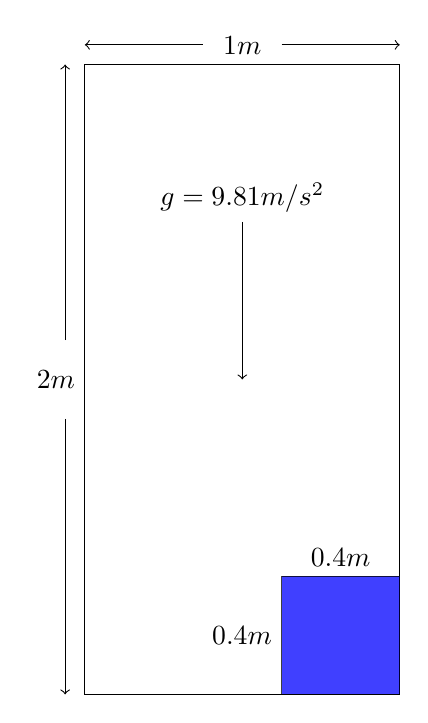
\begin{tikzpicture}
	\draw (0,0) rectangle (4,8);
	\filldraw[fill=blue,opacity=0.75,draw=black] (2.5,0) rectangle (4,1.5);
	\draw[->] (2,6) -- (2,4);
	\node[above] at (2,6) {$g=9.81m/s^2$};
	\node[above] at (3.25,1.5) {$0.4m$};
	\node[left] at (2.5,0.75) {$0.4m$};
	\draw[->] (1.5,8.25) -- (0,8.25);
	\draw[->] (2.5,8.25) -- (4,8.25);
	\node[above] at (2,8) {$1m$};
	\draw[->] (-0.25,3.5) -- (-0.25,0);
	\draw[->] (-0.25,4.5) -- (-0.25,8);
	\node[left] at (0,4) {$2m$};
\end{tikzpicture}
\caption{Schematic of the initial condition.}
\end{figure}

\noindent
The pressure in the water is given by the following equation,

\begin{gather*}
	P=K\times(J^{-\gamma} - 1)
\end{gather*}

\noindent
where $K$ is the low-pressure bulk modulus of the fluid, and $J$ is the determinant of the deformation gradient, while $\gamma=7$ was used throughout these simulations.

\section{Simulation Environment Setup}
This simulation is implemented on Ubuntu 14.04 LTS OS, computing using Uintah 1.6.0 and visualizing the result data by VisIt 2.9.2.

\subsection{Uintah Installation and Configuration}
Uintah is a set of software components and libraries that facilitate the solution of partial differential equations on structured adaptive mesh refinement grids using hundreds to thousands processors\cite{uintahwiki}. To install and configure Uintah software, follow the instruction step by step according to the Uintah Installation Guide\cite{uintahinstallation}.

\subsection{VisIt Installation and Configuration}
VisIt is a free interactive parallel visualization and graphical analysis tool for viewing scientific data on Unix and PC platforms\cite{visitwiki}. Download the VisIt source code and build it following the instruction\cite{visitbuild}. Here is some configuration code:

\begin{lstlisting}[frame=shadowbox,breaklines=true,basicstyle=\ttfamily\small]
sudo env PAR_INCLUDE=-I/usr/local/include PAR_COMPILER=/usr/local/bin/mpic++ PAR_COMPILER_CXX=/usr/local/bin/mipcxx ../src/svn_bin/build_visit -console -thirdparty-path ~/Projects/visit-2.9.2/thirdparty -no-visit -icet -parallel -fortran -alt-uintah-dir ~/Projects/uintah-1.6.0/dbg
\end{lstlisting}

\section{Simulation Specifics}
Component used: MPM\\
Input file name: mpmproblem.ups\\
Command used to run input file: sus /path/to/mpmproblem.ups\\
Simulation Domain: $1.0m \times 2.0m \times axisymmetric$\\
Cell Size: $1.0cm \times 1.0cm$\\
Particles per Cell: $2 \times 2$\\
Bulk Modulus: 15000.0Pa\\
Viscosity: 500cP\\
CFL number: 0.2\\
Physical time simulated: 0.321004 seconds

\section{Uintah Code}
\begin{lstlisting}[frame=shadowbox,breaklines=true,basicstyle=\ttfamily\small]
<?xml version='1.0' encoding='ISO-8859-1' ?>
<Uintah_specification>
	<Meta>
		<title>MPM Problem Simulation</title>
	</Meta>

	<SimulationComponent type="mpm" />

	<Time>
		<maxTime>0.5</maxTime>
		<initTime>0.0</initTime>
		<delt_min>0.00001</delt_min>
		<delt_max>0.001</delt_max>
		<max_Timesteps>3000000</max_Timesteps>
		<timestep_multiplier>0.2</timestep_multiplier>
	</Time>

	<Grid>
	<BoundaryConditions>
	<Face side="x-">
	<BCType id="all" var="symmetry" label="Symmetric"></BCType>
	</Face>

	<Face side="x+">
	<BCType id="all" var="symmetry" label="Symmetric"></BCType>
	</Face>

	<Face side="y-">
	<BCType id="all" var="symmetry" label="Symmetric"></BCType>
	</Face>

	<Face side="y+">
	<BCType id="all" var="symmetry" label="Symmetric"></BCType>
	</Face>

	<Face side="z-">
	<BCType id="all" var="symmetry" label="Symmetric"></BCType>
	</Face>

	<Face side="z+">
	<BCType id="all" var="symmetry" label="Symmetric"></BCType>
	</Face>
	</BoundaryConditions>
		
	<Level>
	<Box label = "domain">
	<lower>[0.0, 0.0, 0.0]</lower>
	<upper>[1.0, 2.0, 0.1]</upper>
	<extraCells>[1,1,1]</extraCells>
	<patches>[1,1,1]</patches>
	</Box>
	<spacing>[0.01, 0.01, 0.01]</spacing>
	</Level>
	</Grid>


	<DataArchiver>
		<filebase>problem.uda</filebase>
		<outputInterval>.001</outputInterval>
		<save label="p.x"/>
		<save label="p.velocity"/>
		<save label="p.volume"/>
		<save label="p.size"/>
		<save label="p.temperature"/>
		<save label="p.deformationMeasure"/>
		<save label="p.stress"/>
		<save label="g.mass"/>
		<save label="g.stressFS"/>
		<save label="g.velocity"/>
		<save label="g.velocity_star"/>
	</DataArchiver>

	<MPM>
		<time_integrator>explicit</time_integrator>
		<interpolator>gimp</interpolator>
	</MPM>

	<PhysicalConstants>
		<gravity>[0,-9.81,0]</gravity>
	</PhysicalConstants>

	<MaterialProperties>
		<MPM>
		<material>
		<density>1000.0</density>
		<constitutive_model type="water">
		<bulk_modulus>15000.0</bulk_modulus>
		<viscosity>0.5</viscosity>
		<gamma>7.0</gamma>
		</constitutive_model>

		<thermal_conductivity>0.0</thermal_conductivity>

		<specific_heat>5</specific_heat>

		<geom_object>
		<box label = "particles">
		<min>[0.6, 0.0, 0.0]</min>
		<max>[1.0, 0.4, 0.1]</max>
		</box>
		<res>[2,2,2]</res>
		<velocity>[0.0, -9.81, 0.0]</velocity>
		<temperature>12</temperature>
		</geom_object>
		</material>
		</MPM>
	</MaterialProperties>

</Uintah_specification>
\end{lstlisting}

\section{Results}
\begin{figure}[H]
  \centering
  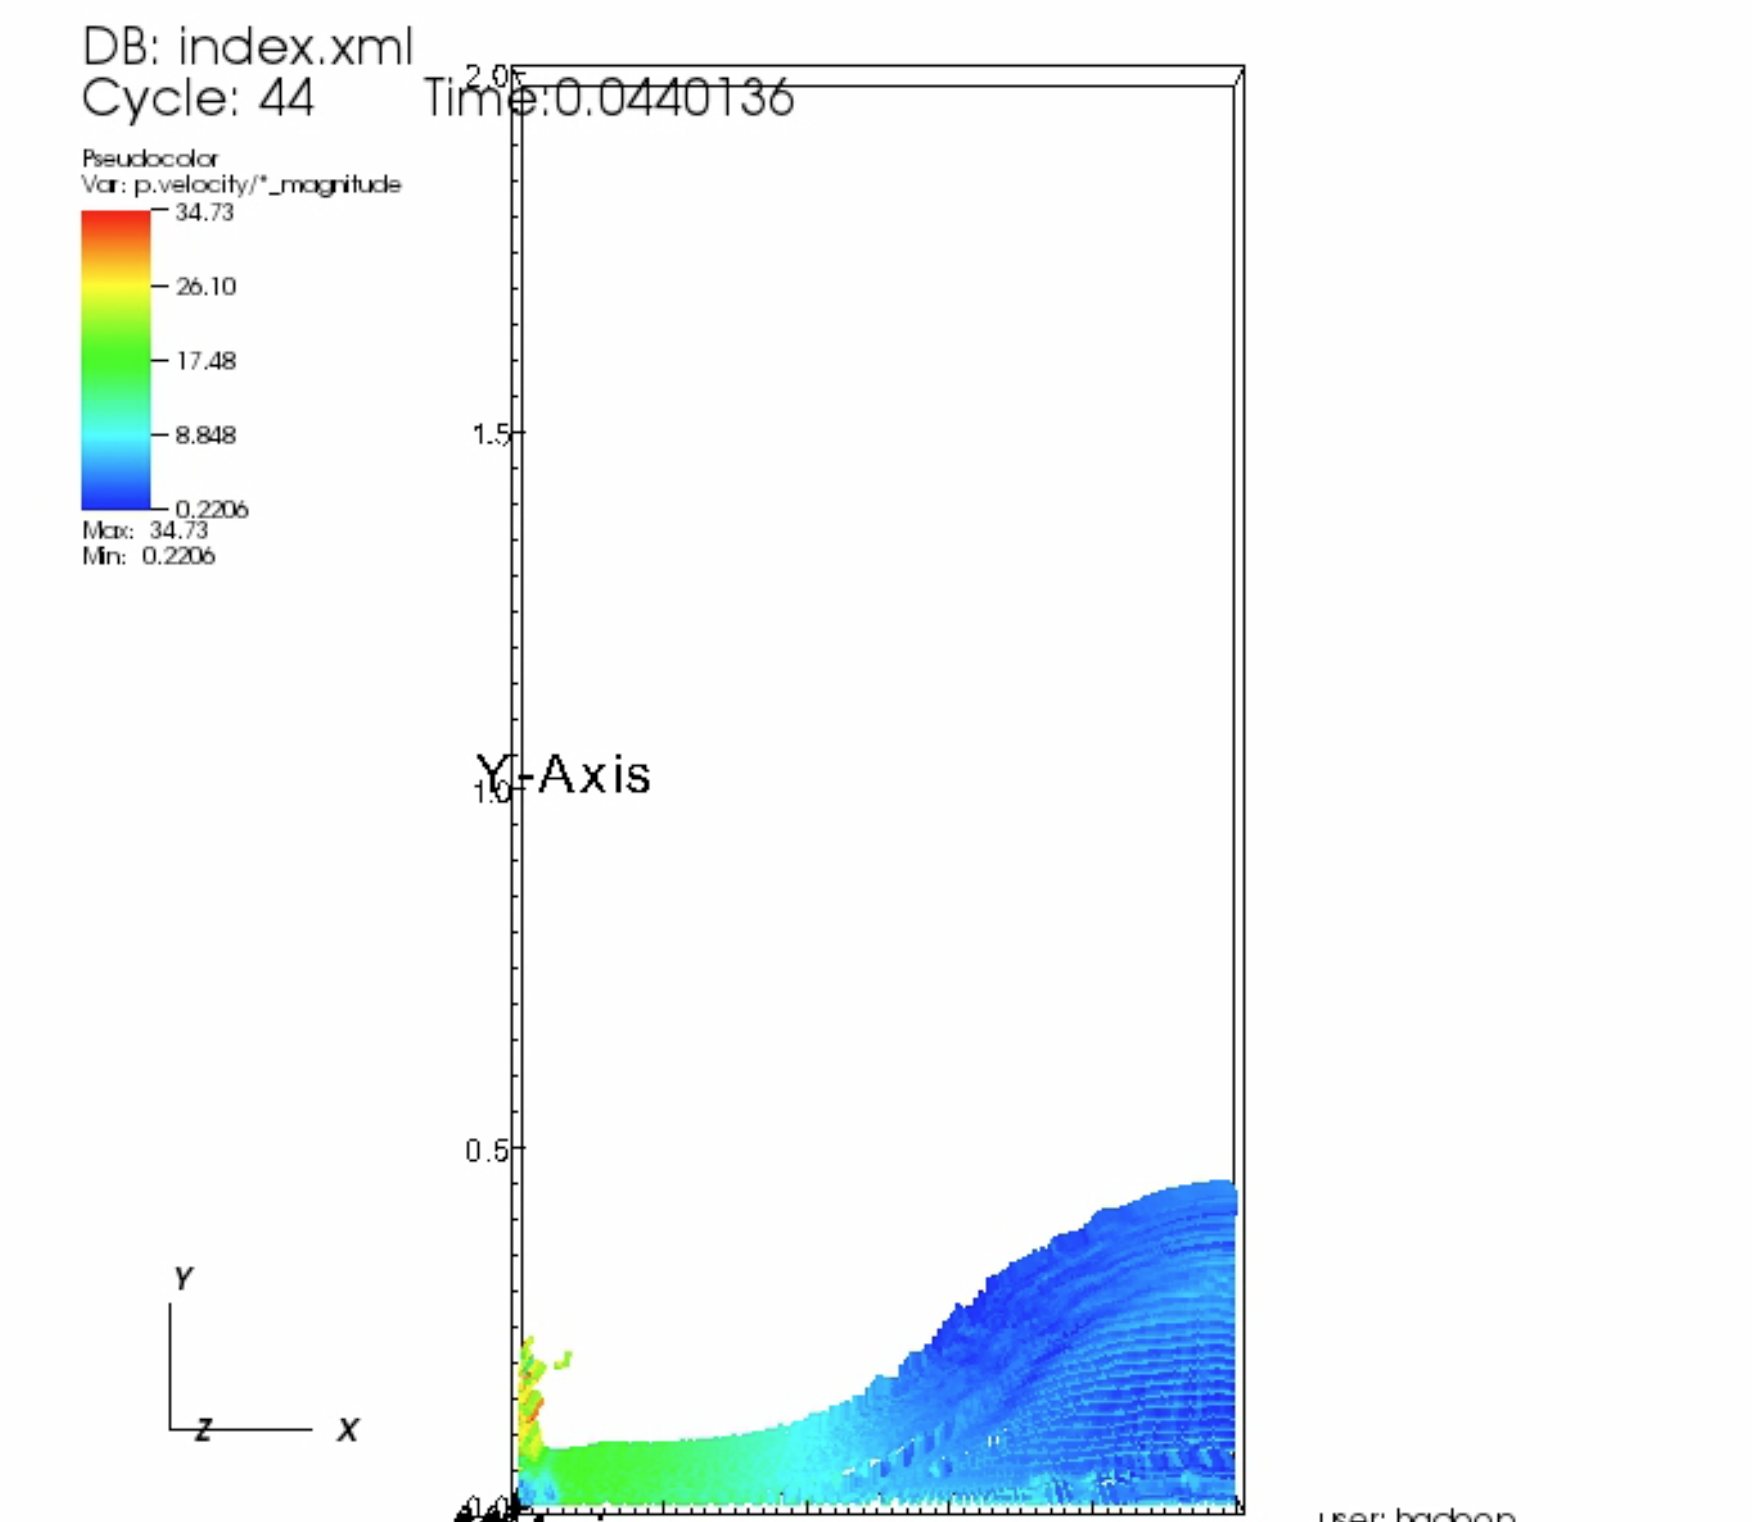
\includegraphics[width=3.0in]{images/1}
  \caption{Initially stable fluid}
\end{figure}
Figure 2 shows the initially simulation of the fluid is stable, with particles colored by the magnitude of their velocity.

\begin{figure}[H]
	\centering
	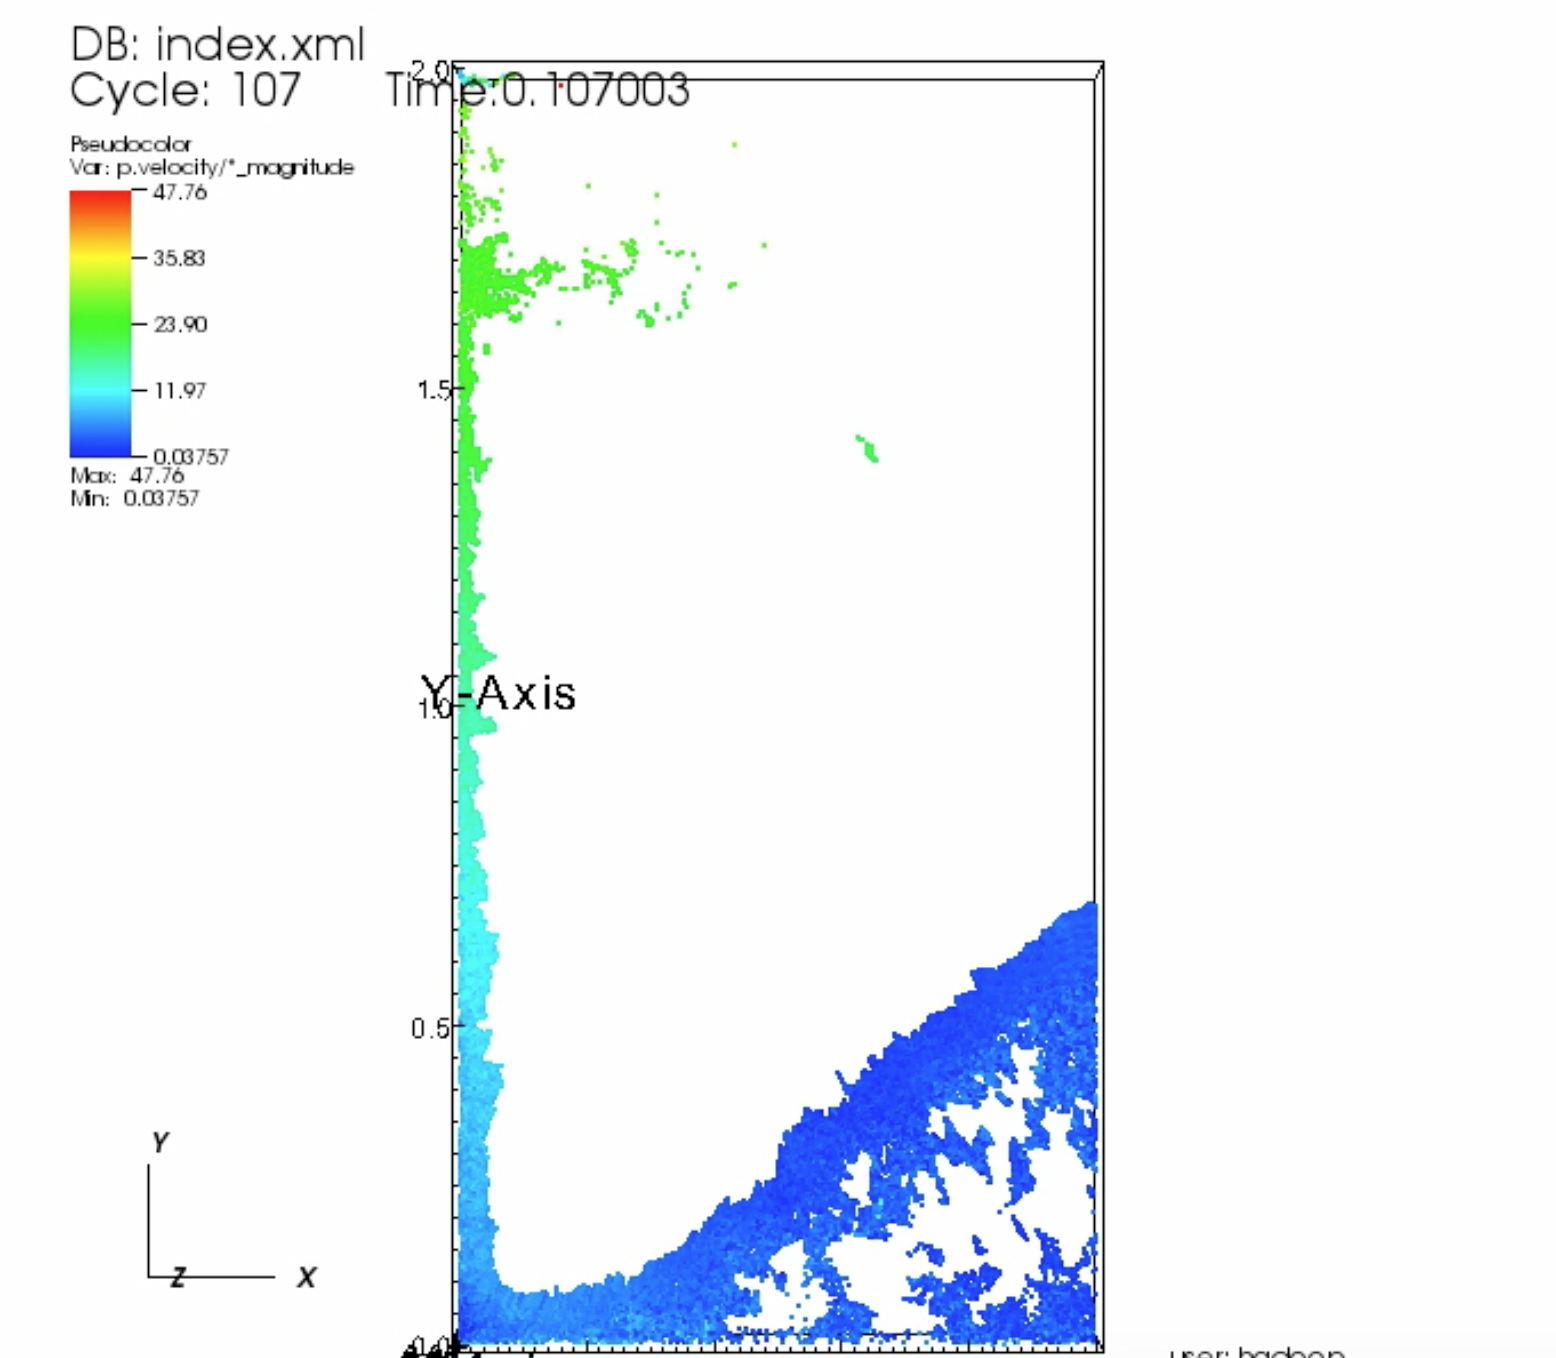
\includegraphics[width=3.0in]{images/2}
	\caption{State of fluid after a few time steps}
\end{figure}
Figure 3 shows the fluid state becomes unstable after a few time steps.

\begin{figure}[H]
	\centering
	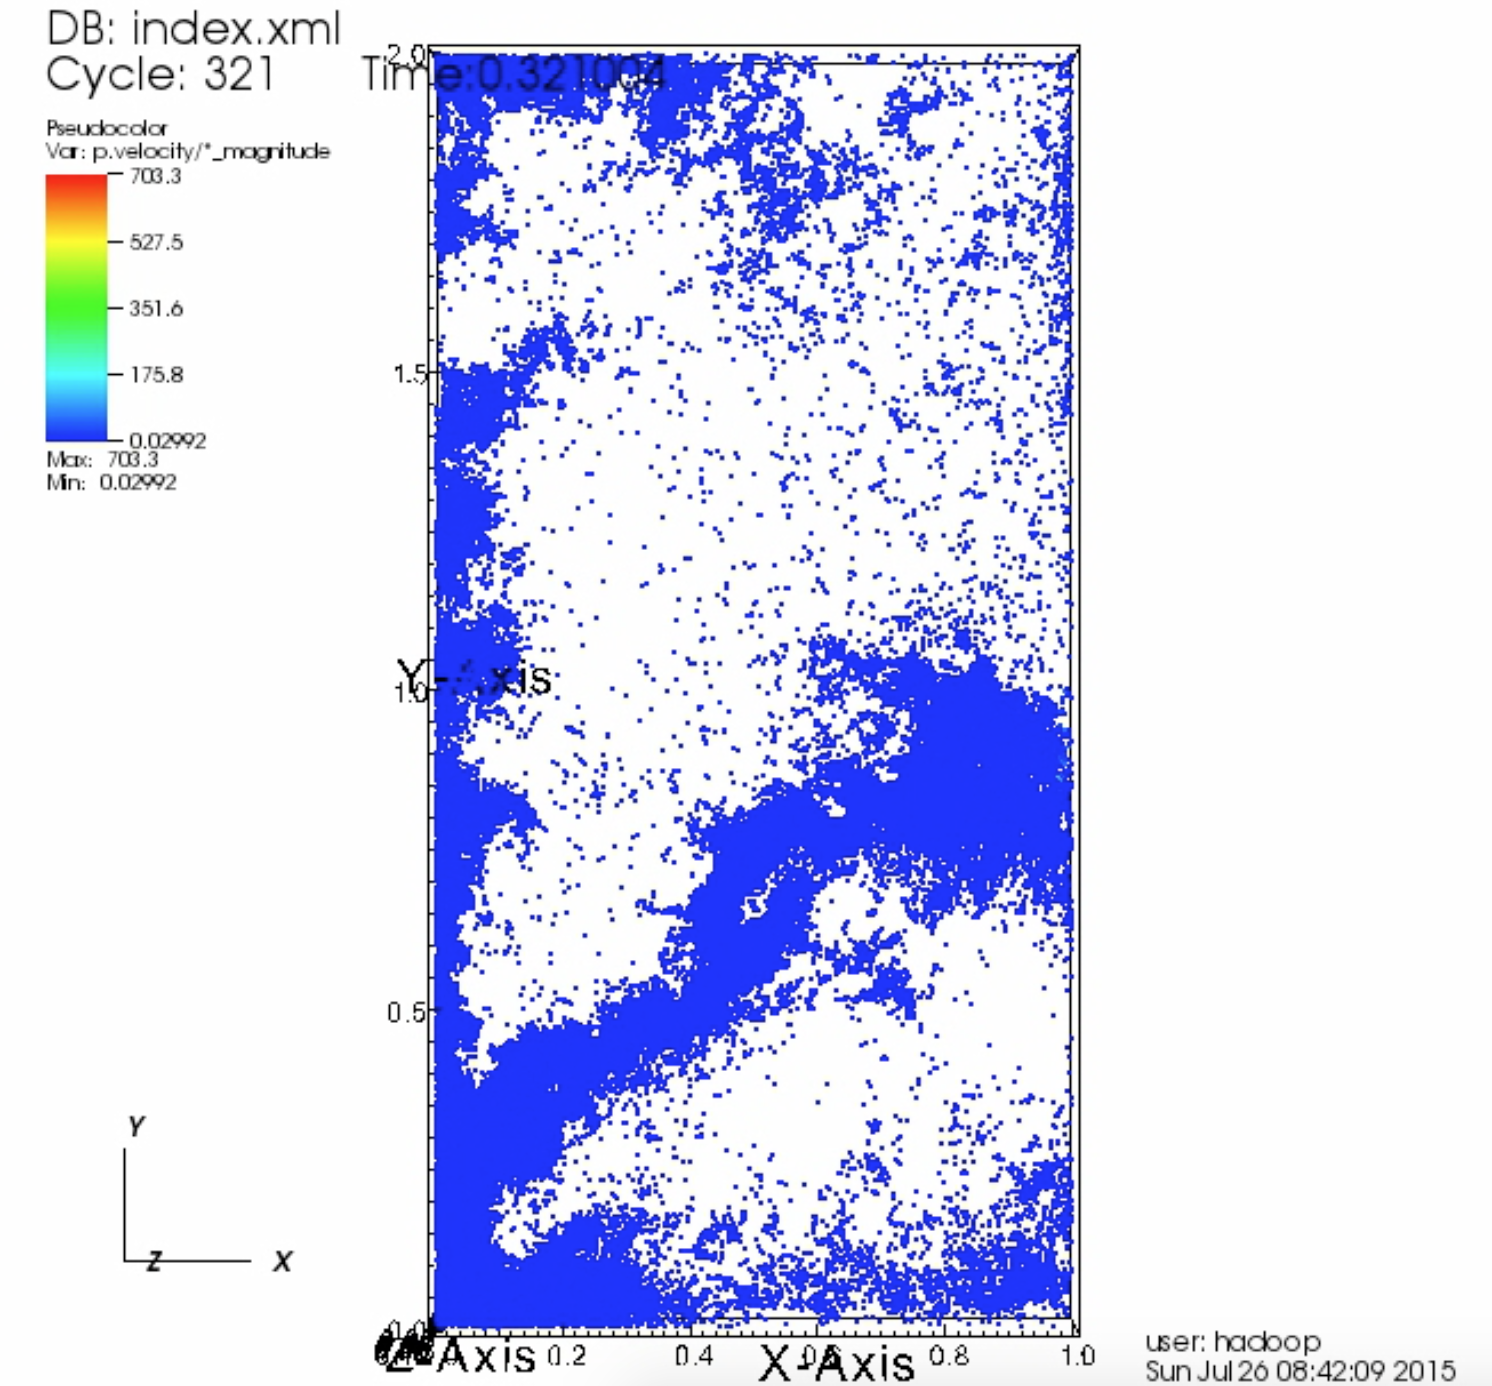
\includegraphics[width=3.0in]{images/3}
	\caption{Particles blow out}
\end{figure}
Figure 4 shows after 0.3 seconds simulation, most of the particles are blown out in the closed domain with an unstable fluid state.

\section{Conclusion}
\begin{enumerate}
	\item In this problem, the pressure in the water is given by an equation of state described as $P=K\times(J^{-\gamma} - 1)$, where $K$ is the low-pressure bulk modulus of the fluid in which seems more likely a penalization term coefficient. In a small region of computational domain, any subtle difference of density would cause enormous pressure even anomaly huge $\nabla{p}$ depending on the $k$ chosen. MPM\cite{sulsky1994particle}\cite{nguyenmaterial} combines the algorithm of SPH\cite{muller2003particle} in which the pressure term is solved in an explicit method. A better way to avoid the numerical instability problem may include considering using an implicit pressure projection method instead.
	\item In \cite{stomakhin2014augmented}, the study employ the Chorin-style projection which are naturally done on maker and cell(MAC) grids. By introducing an intermediate velocity $u*$, pressure are split from the other forces, taking the divergence, the equation then reduces to a Poisson Equation to solve.
	\item The unstable source may also occur in the information exchanged between particles and grids in MPM. Employing more smooth particle-grids information exchange algorithm should help.
\end{enumerate}

\bibliographystyle{plain}
\nocite{*}
\bibliography{report}
\end{document}